\documentclass{standalone}
\usepackage{tikz}
\usepackage{pgfplots}

\begin{document}
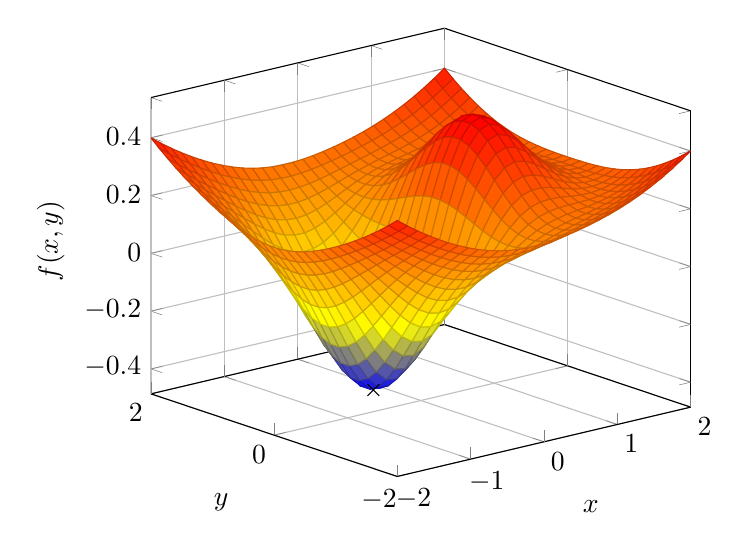
\begin{tikzpicture}
    \begin{axis}[
        xlabel={$x$},
        ylabel={$y$},
        zlabel={$f(x, y)$},
        domain=-2:2,
        y domain=-2:2,
        samples=30,
        view={-40}{20},
        grid=both, % Adiciona grade em ambos os eixos
        %minor tick num=1 % Adiciona linhas de grade menores
    ]
    \addplot3 [surf] {x*exp(-x^2-y^2) + (x^2 + y^2)/20};
    
    % Coordenadas do ponto de mínimo (ajuste conforme necessário)
    \addplot3[only marks, mark=x, mark size=3pt] coordinates {(-1, -0.42, -0.36)};
    \end{axis}
\end{tikzpicture}
\end{document}